\newcommand{\undersetimage}[3]{
    \begin{tikzpicture}
        \node[anchor=south west,inner sep=0] (image) at (0, 0)
            {\includegraphics[width=0.65cm]{#1}};
        \begin{scope}[x={(image.south east)},y={(image.north west)}]
            \node[] at (0.5, #3) {#2};
        \end{scope}
    \end{tikzpicture}
}

\begin{figure*}
\centering
\begin{minipage}[t]{0.55\textwidth}
    \raisebox{2cm}{\textbf{a}}~~~
    \hspace{.2cm}
    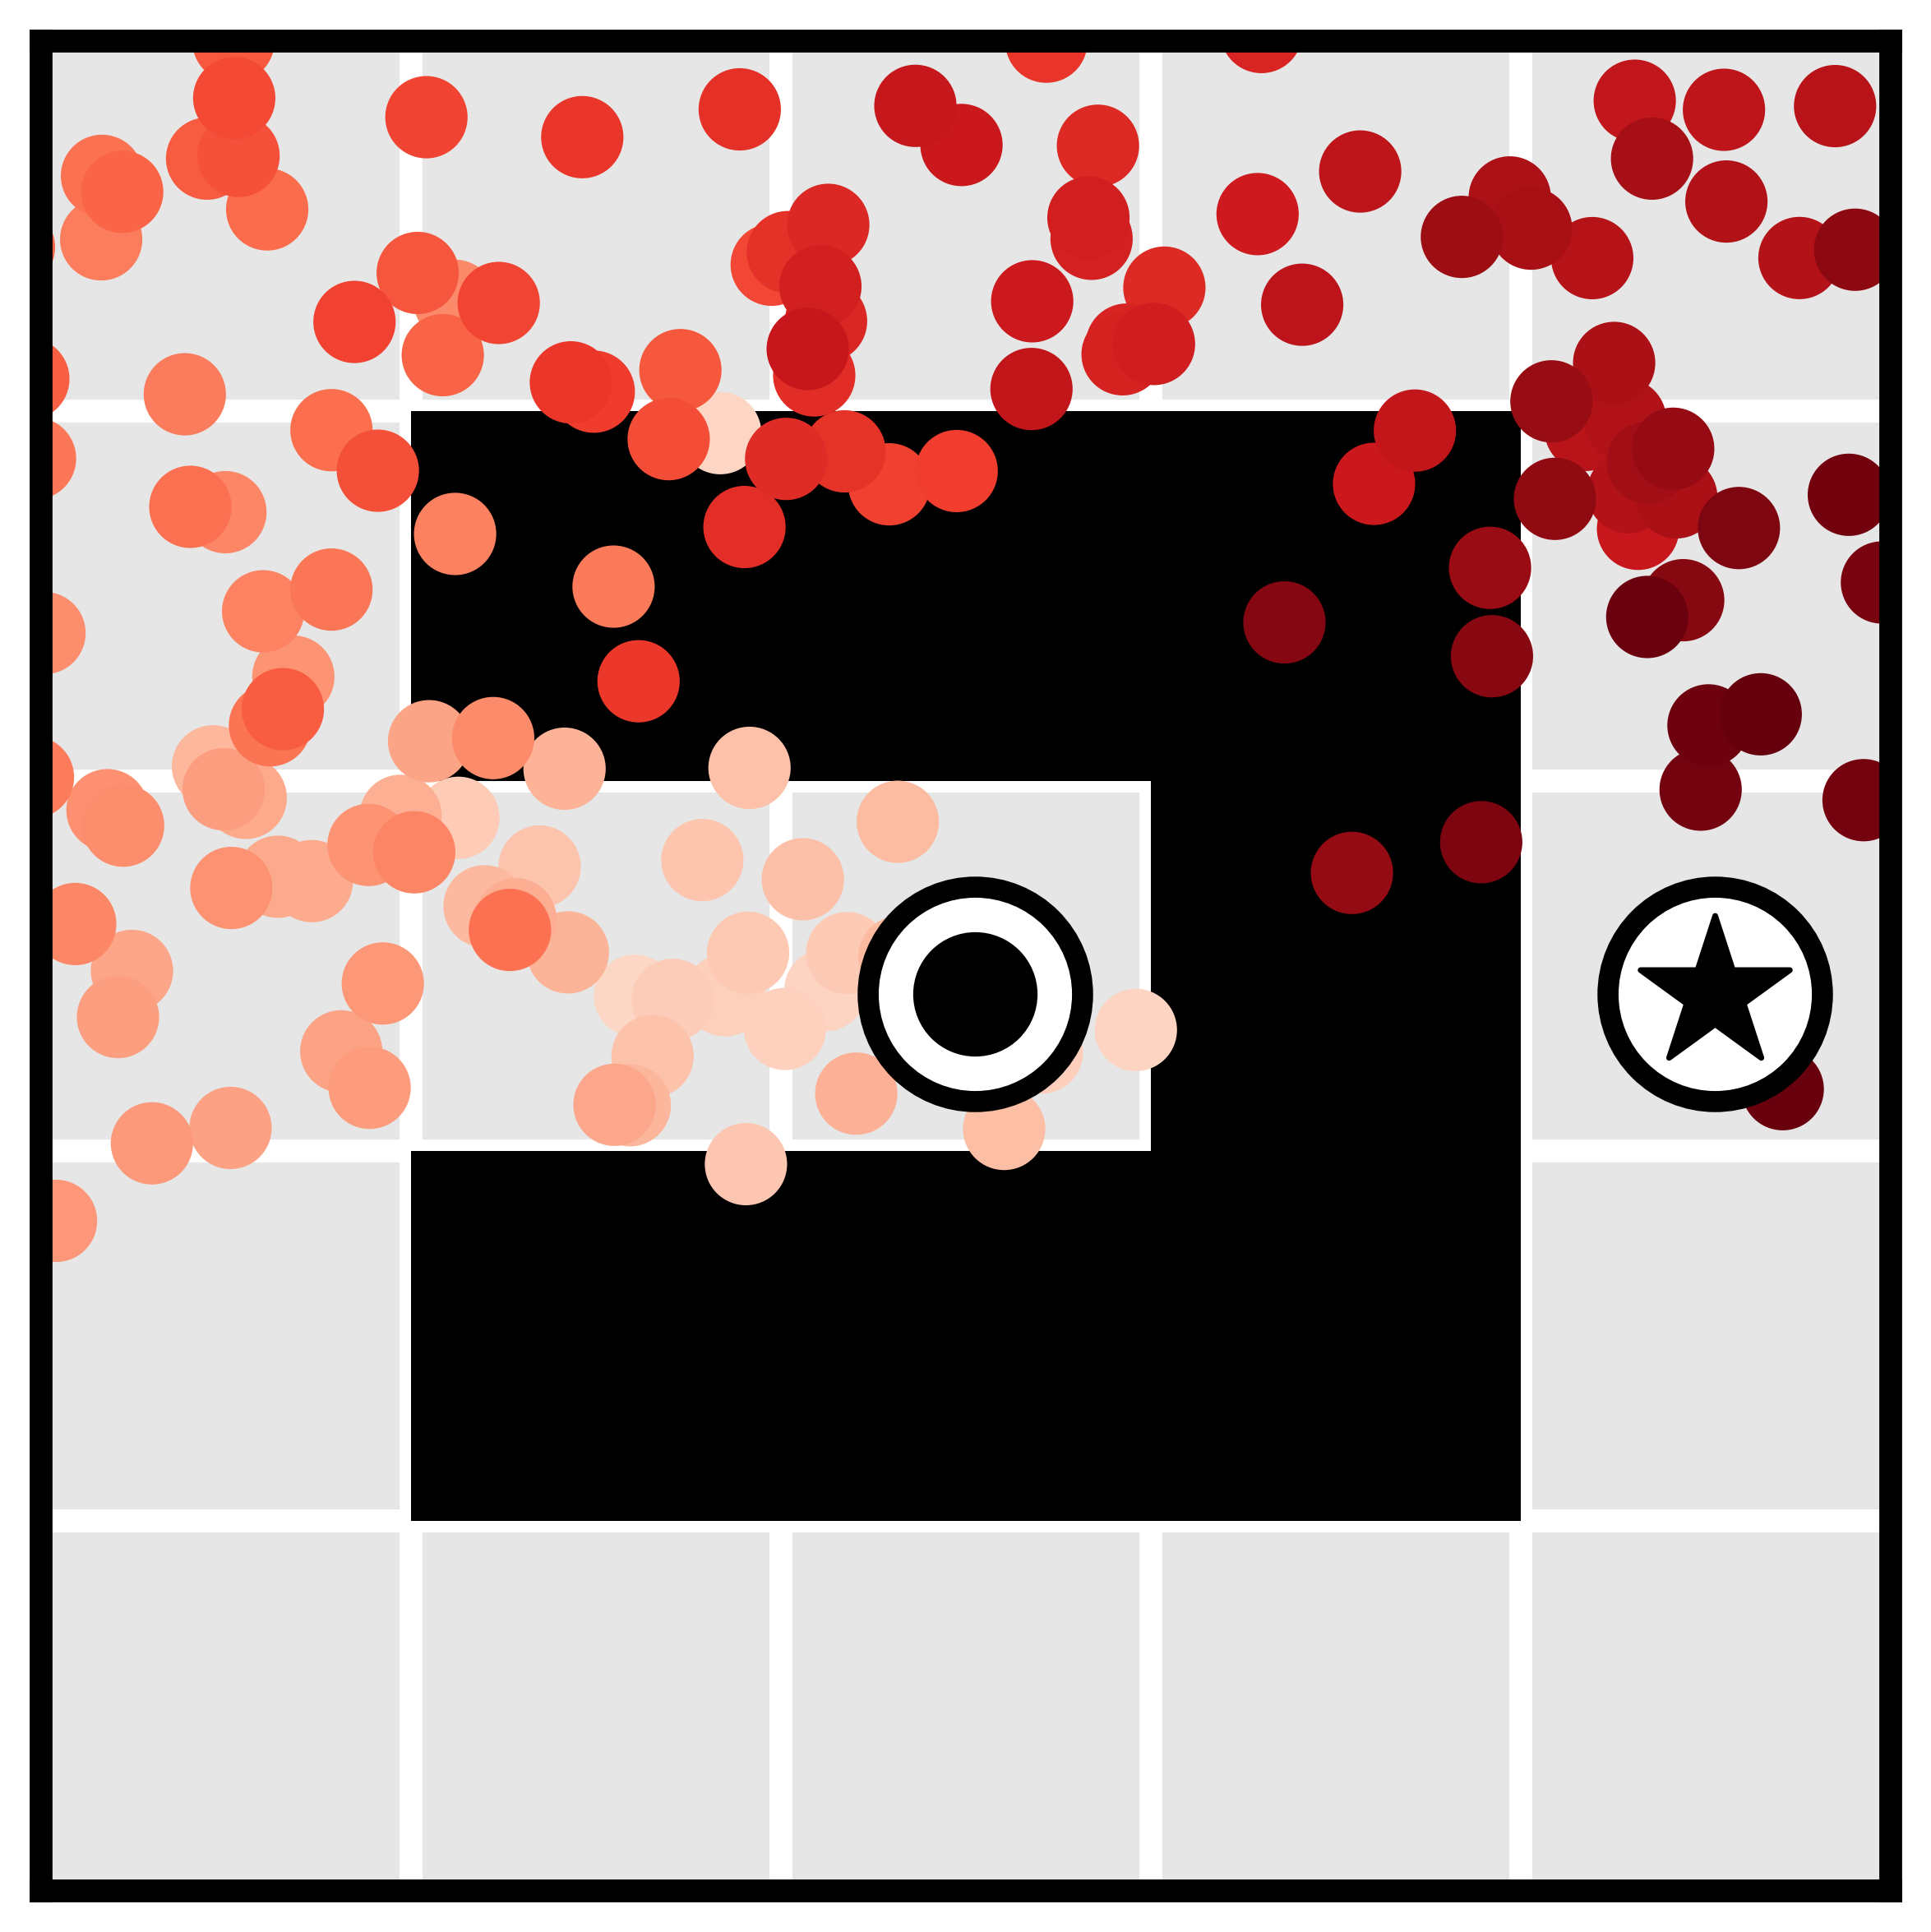
\includegraphics[width=2.5cm]{images/properties/planning_2.png}~
    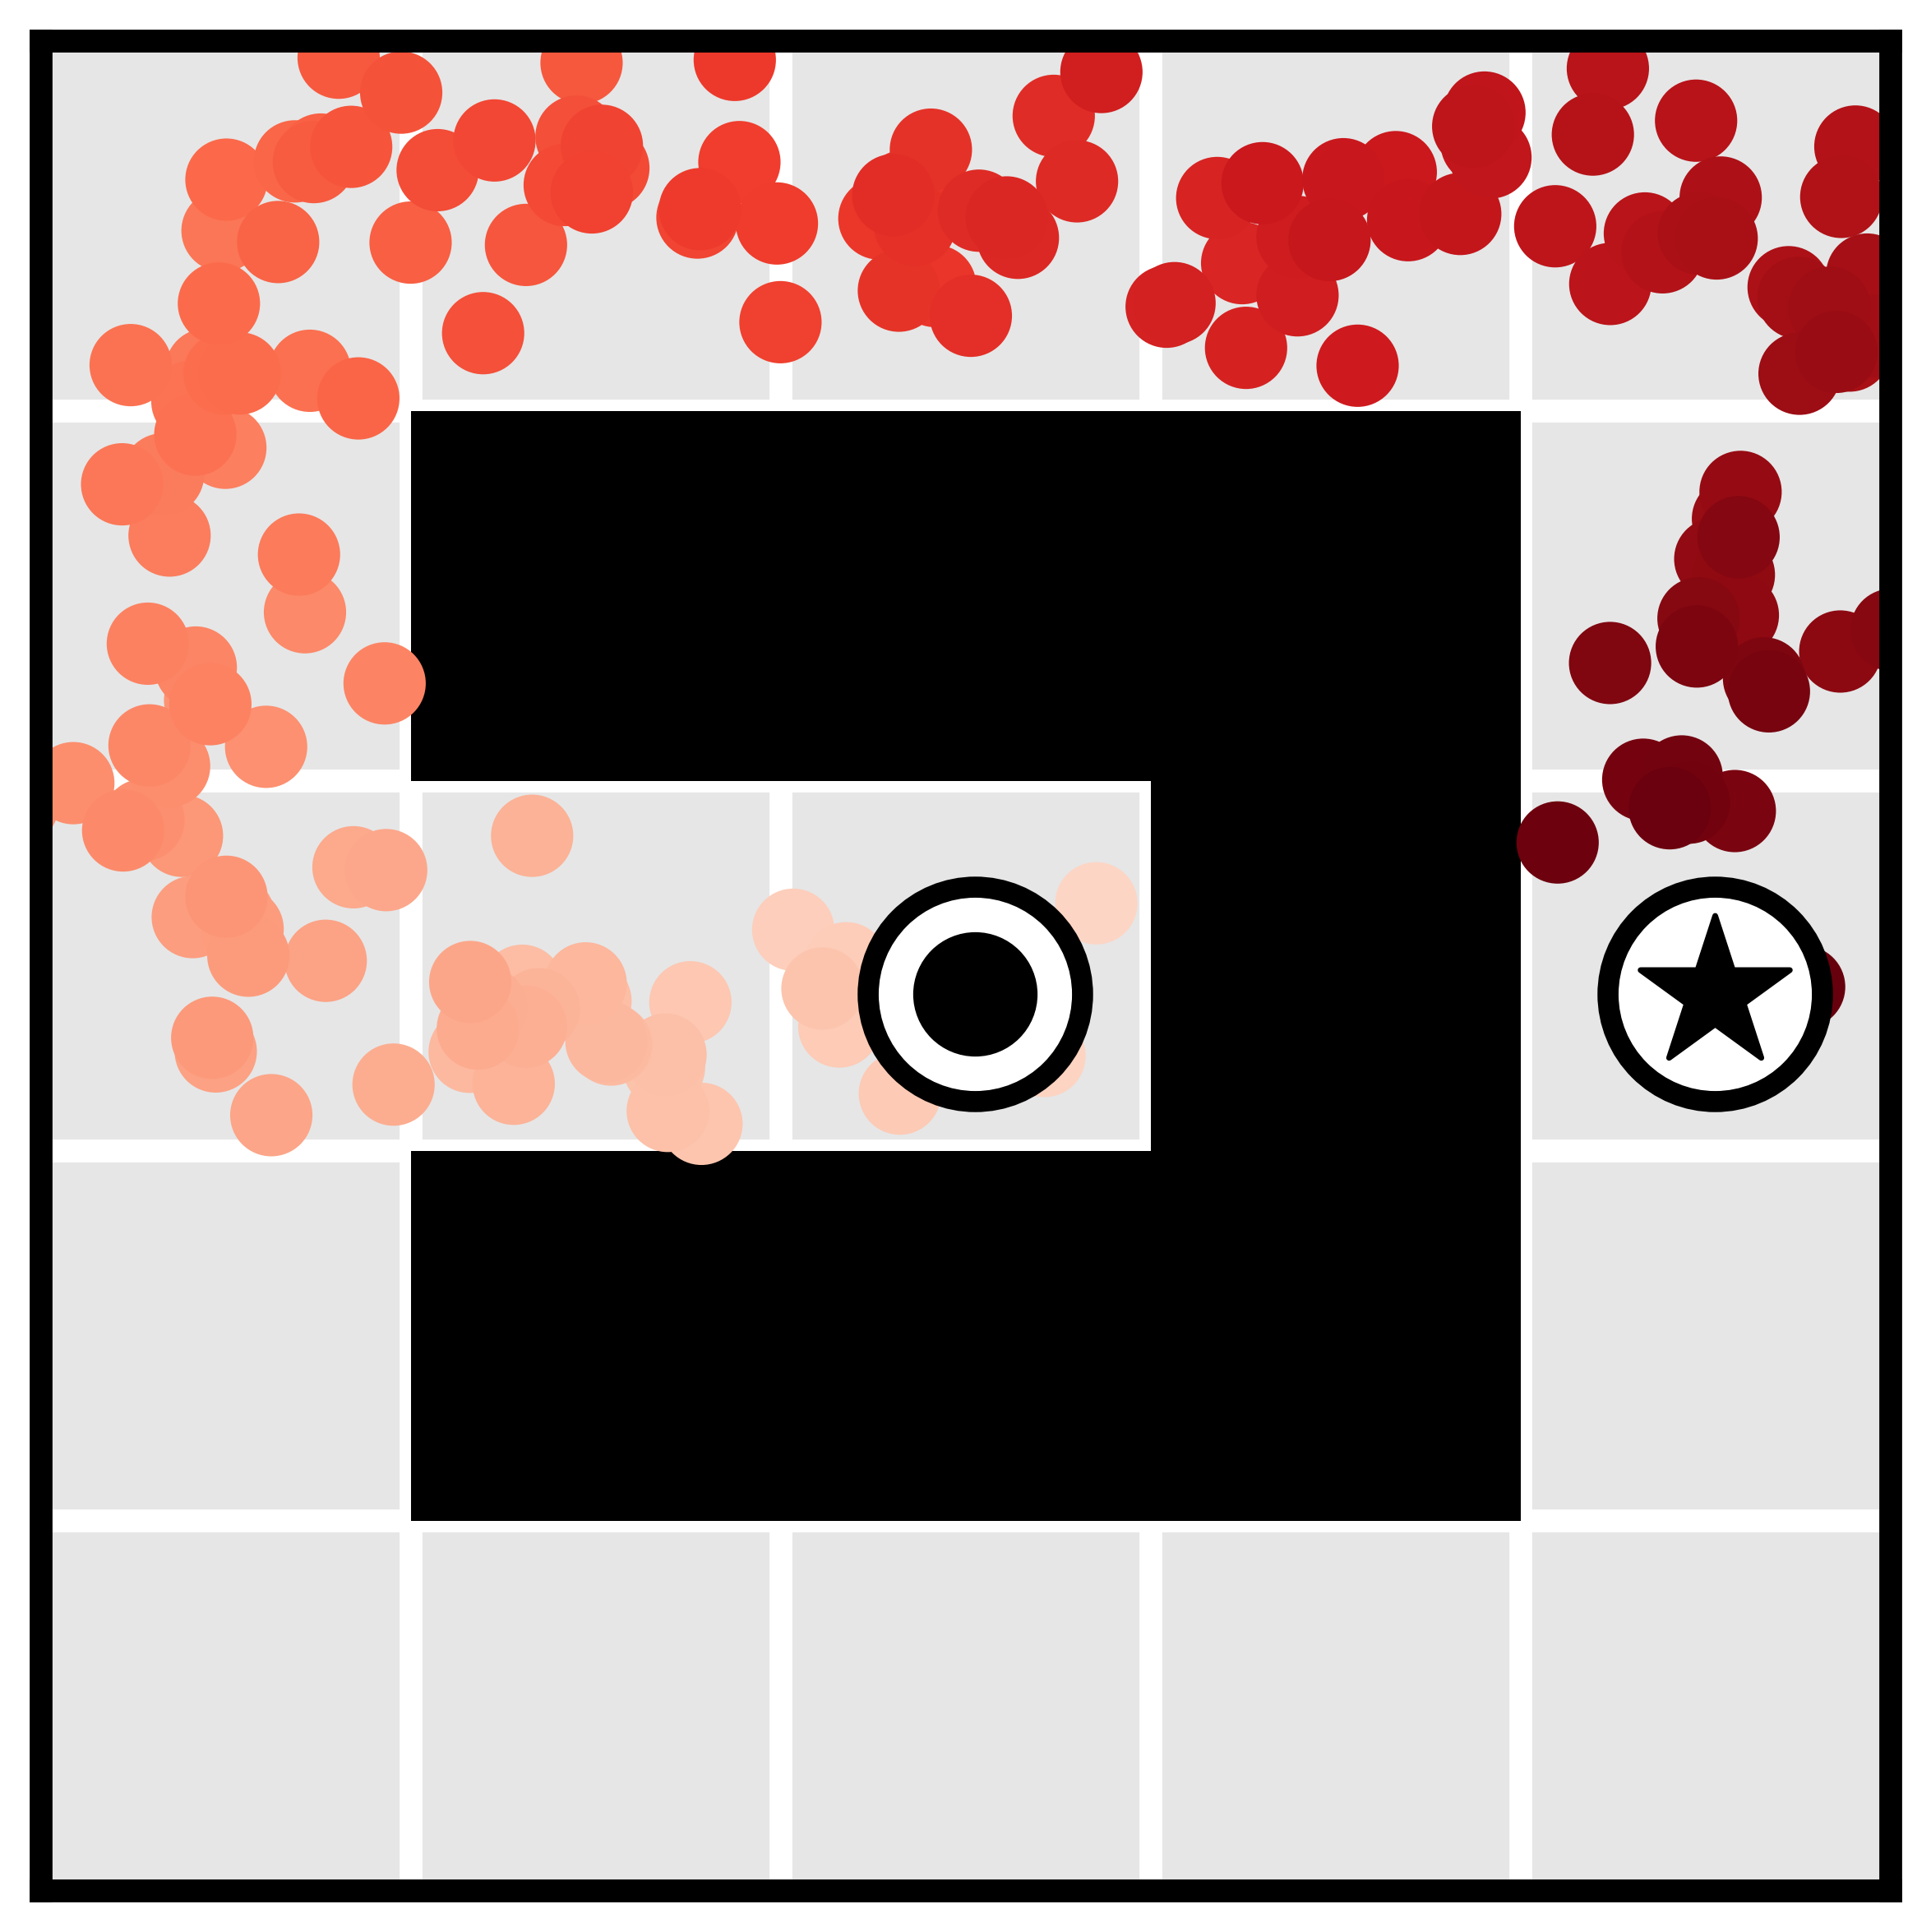
\includegraphics[width=2.5cm]{images/properties/planning_1.png}~
    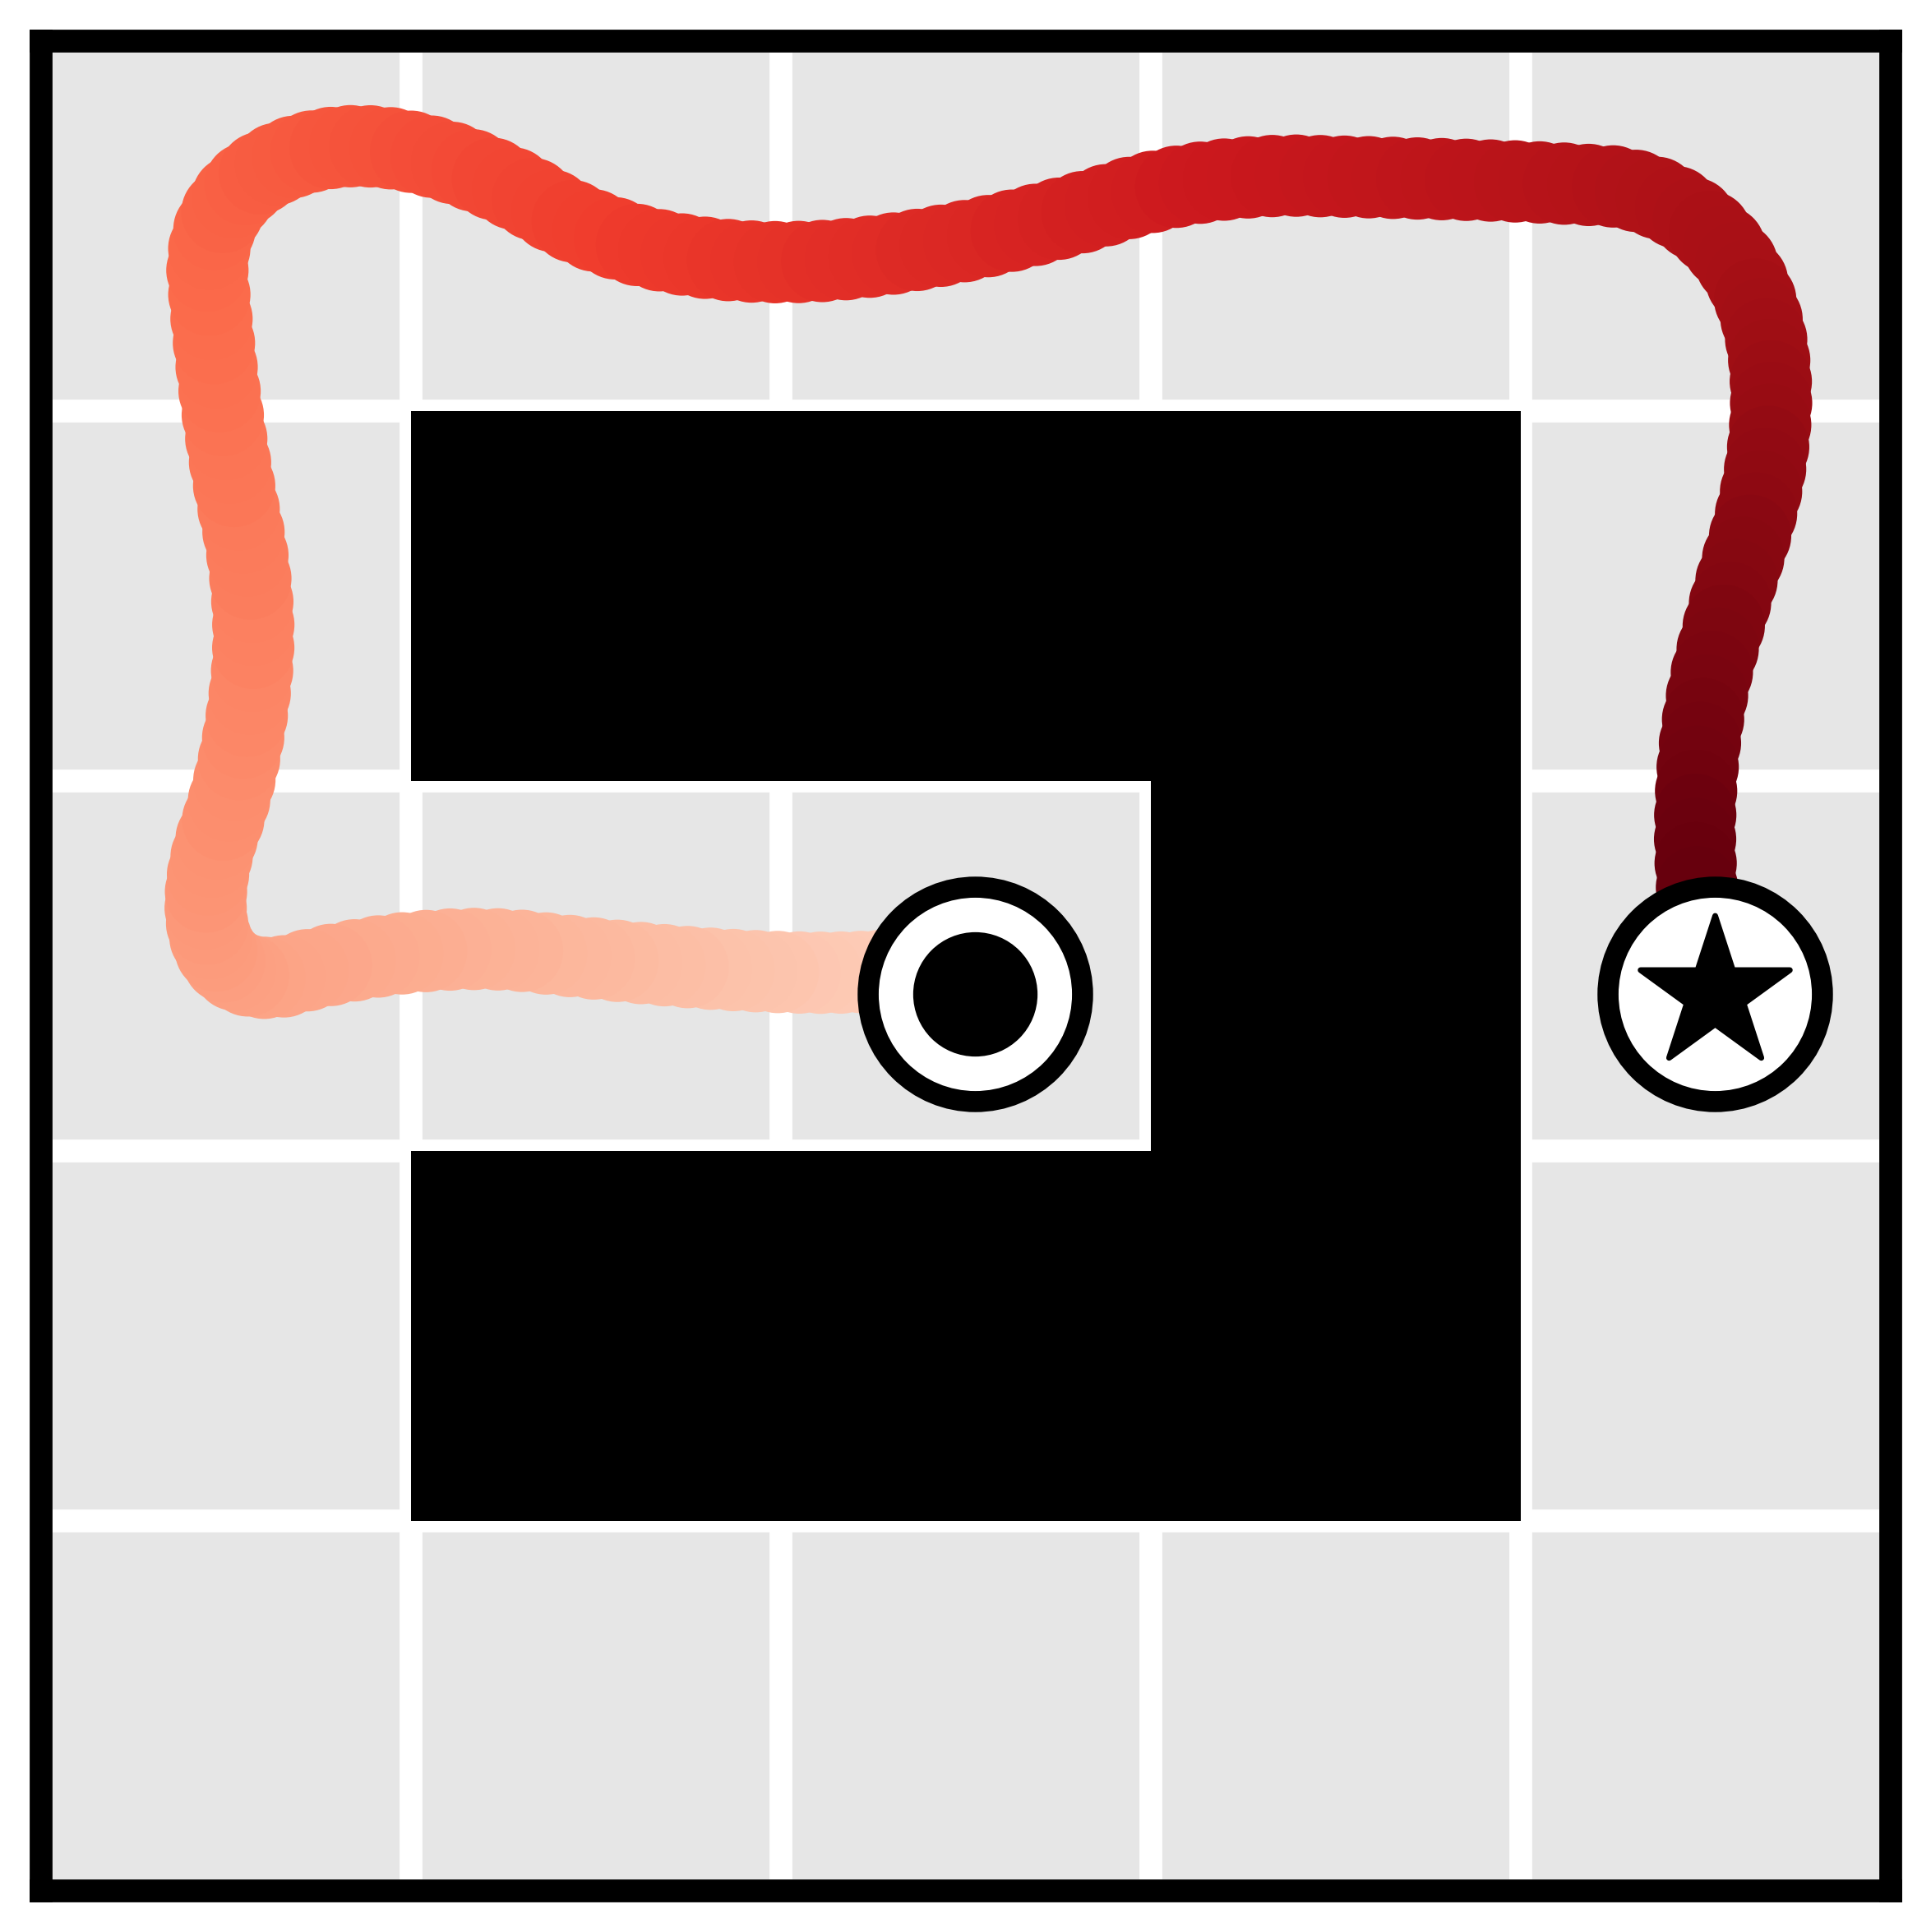
\includegraphics[width=2.5cm]{images/properties/planning_0.png} \\
    \vspace{-.4cm}
    \begin{center}
        \raisebox{.3\height}{denoising}~~
        \tikz \draw [-{Computer Modern Rightarrow[length=1.33mm, width=2mm]}, line width=.2mm] (0,0) -- (3,0); \\
    \end{center}
\end{minipage}%
%%%%
\begin{minipage}[t]{0.35\textwidth}
    \raisebox{2cm}{\textbf{b}}~~~
    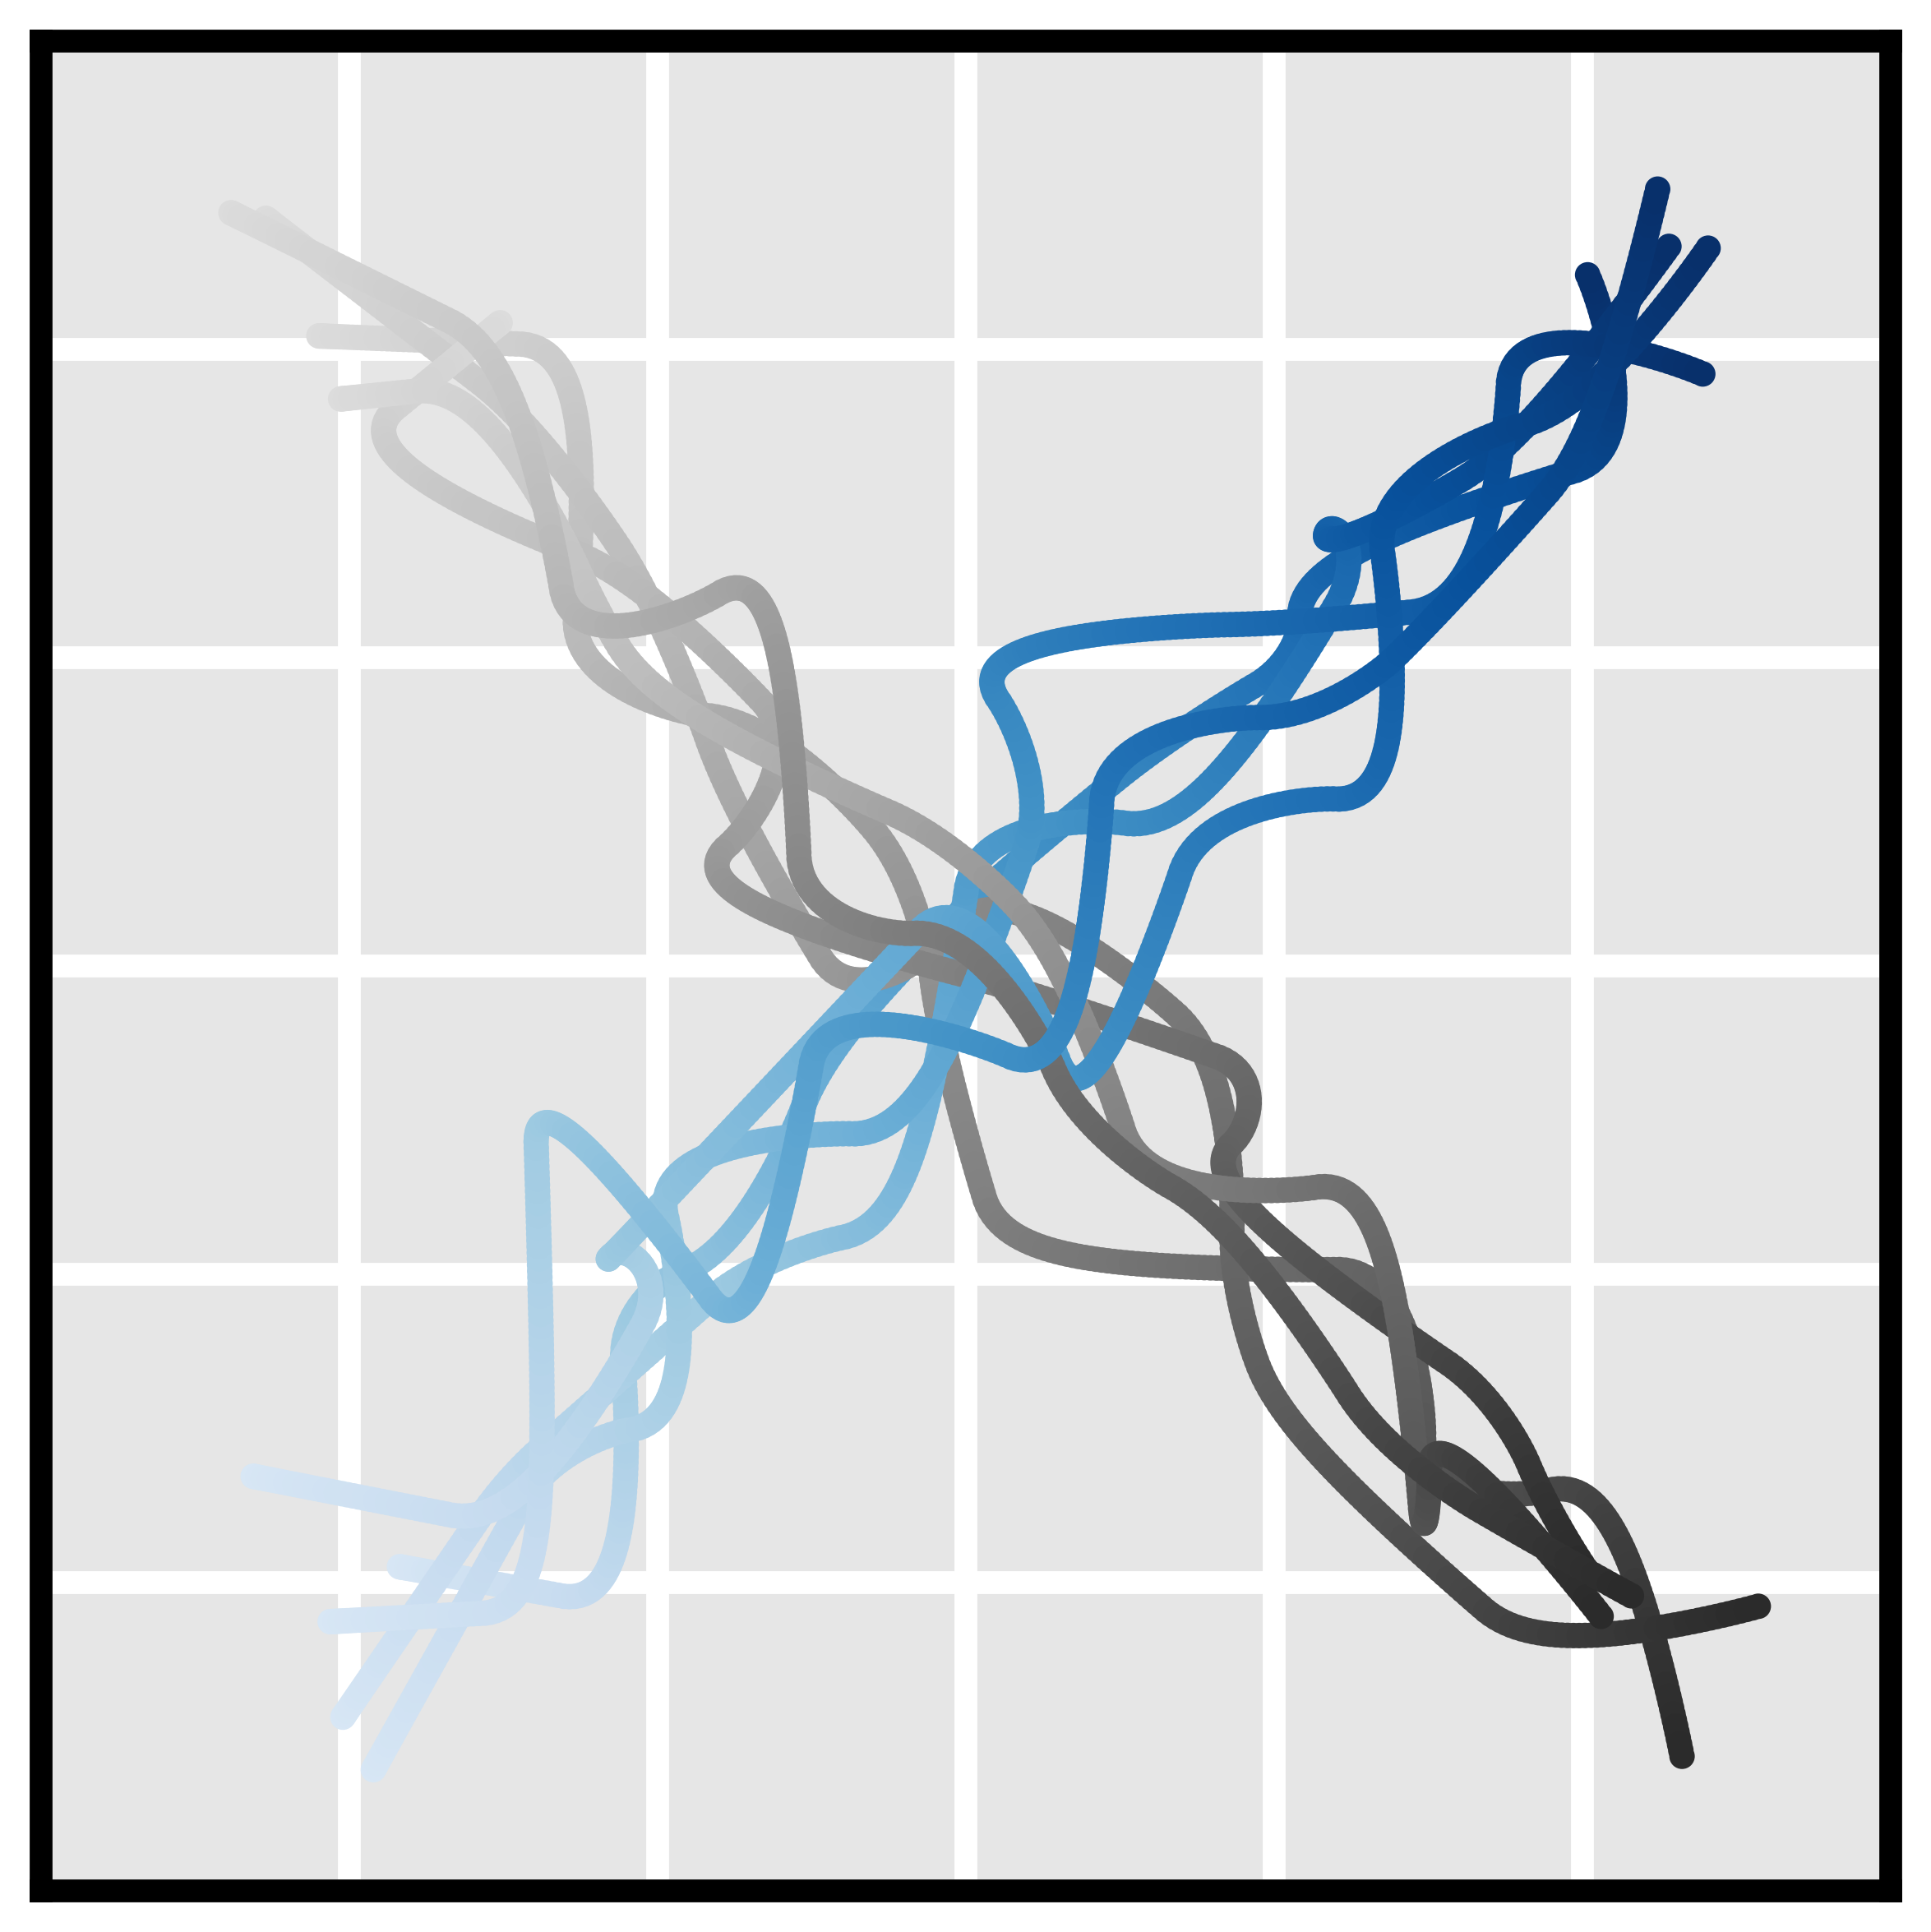
\includegraphics[width=2.5cm]{images/properties/stitching_data.png}~
    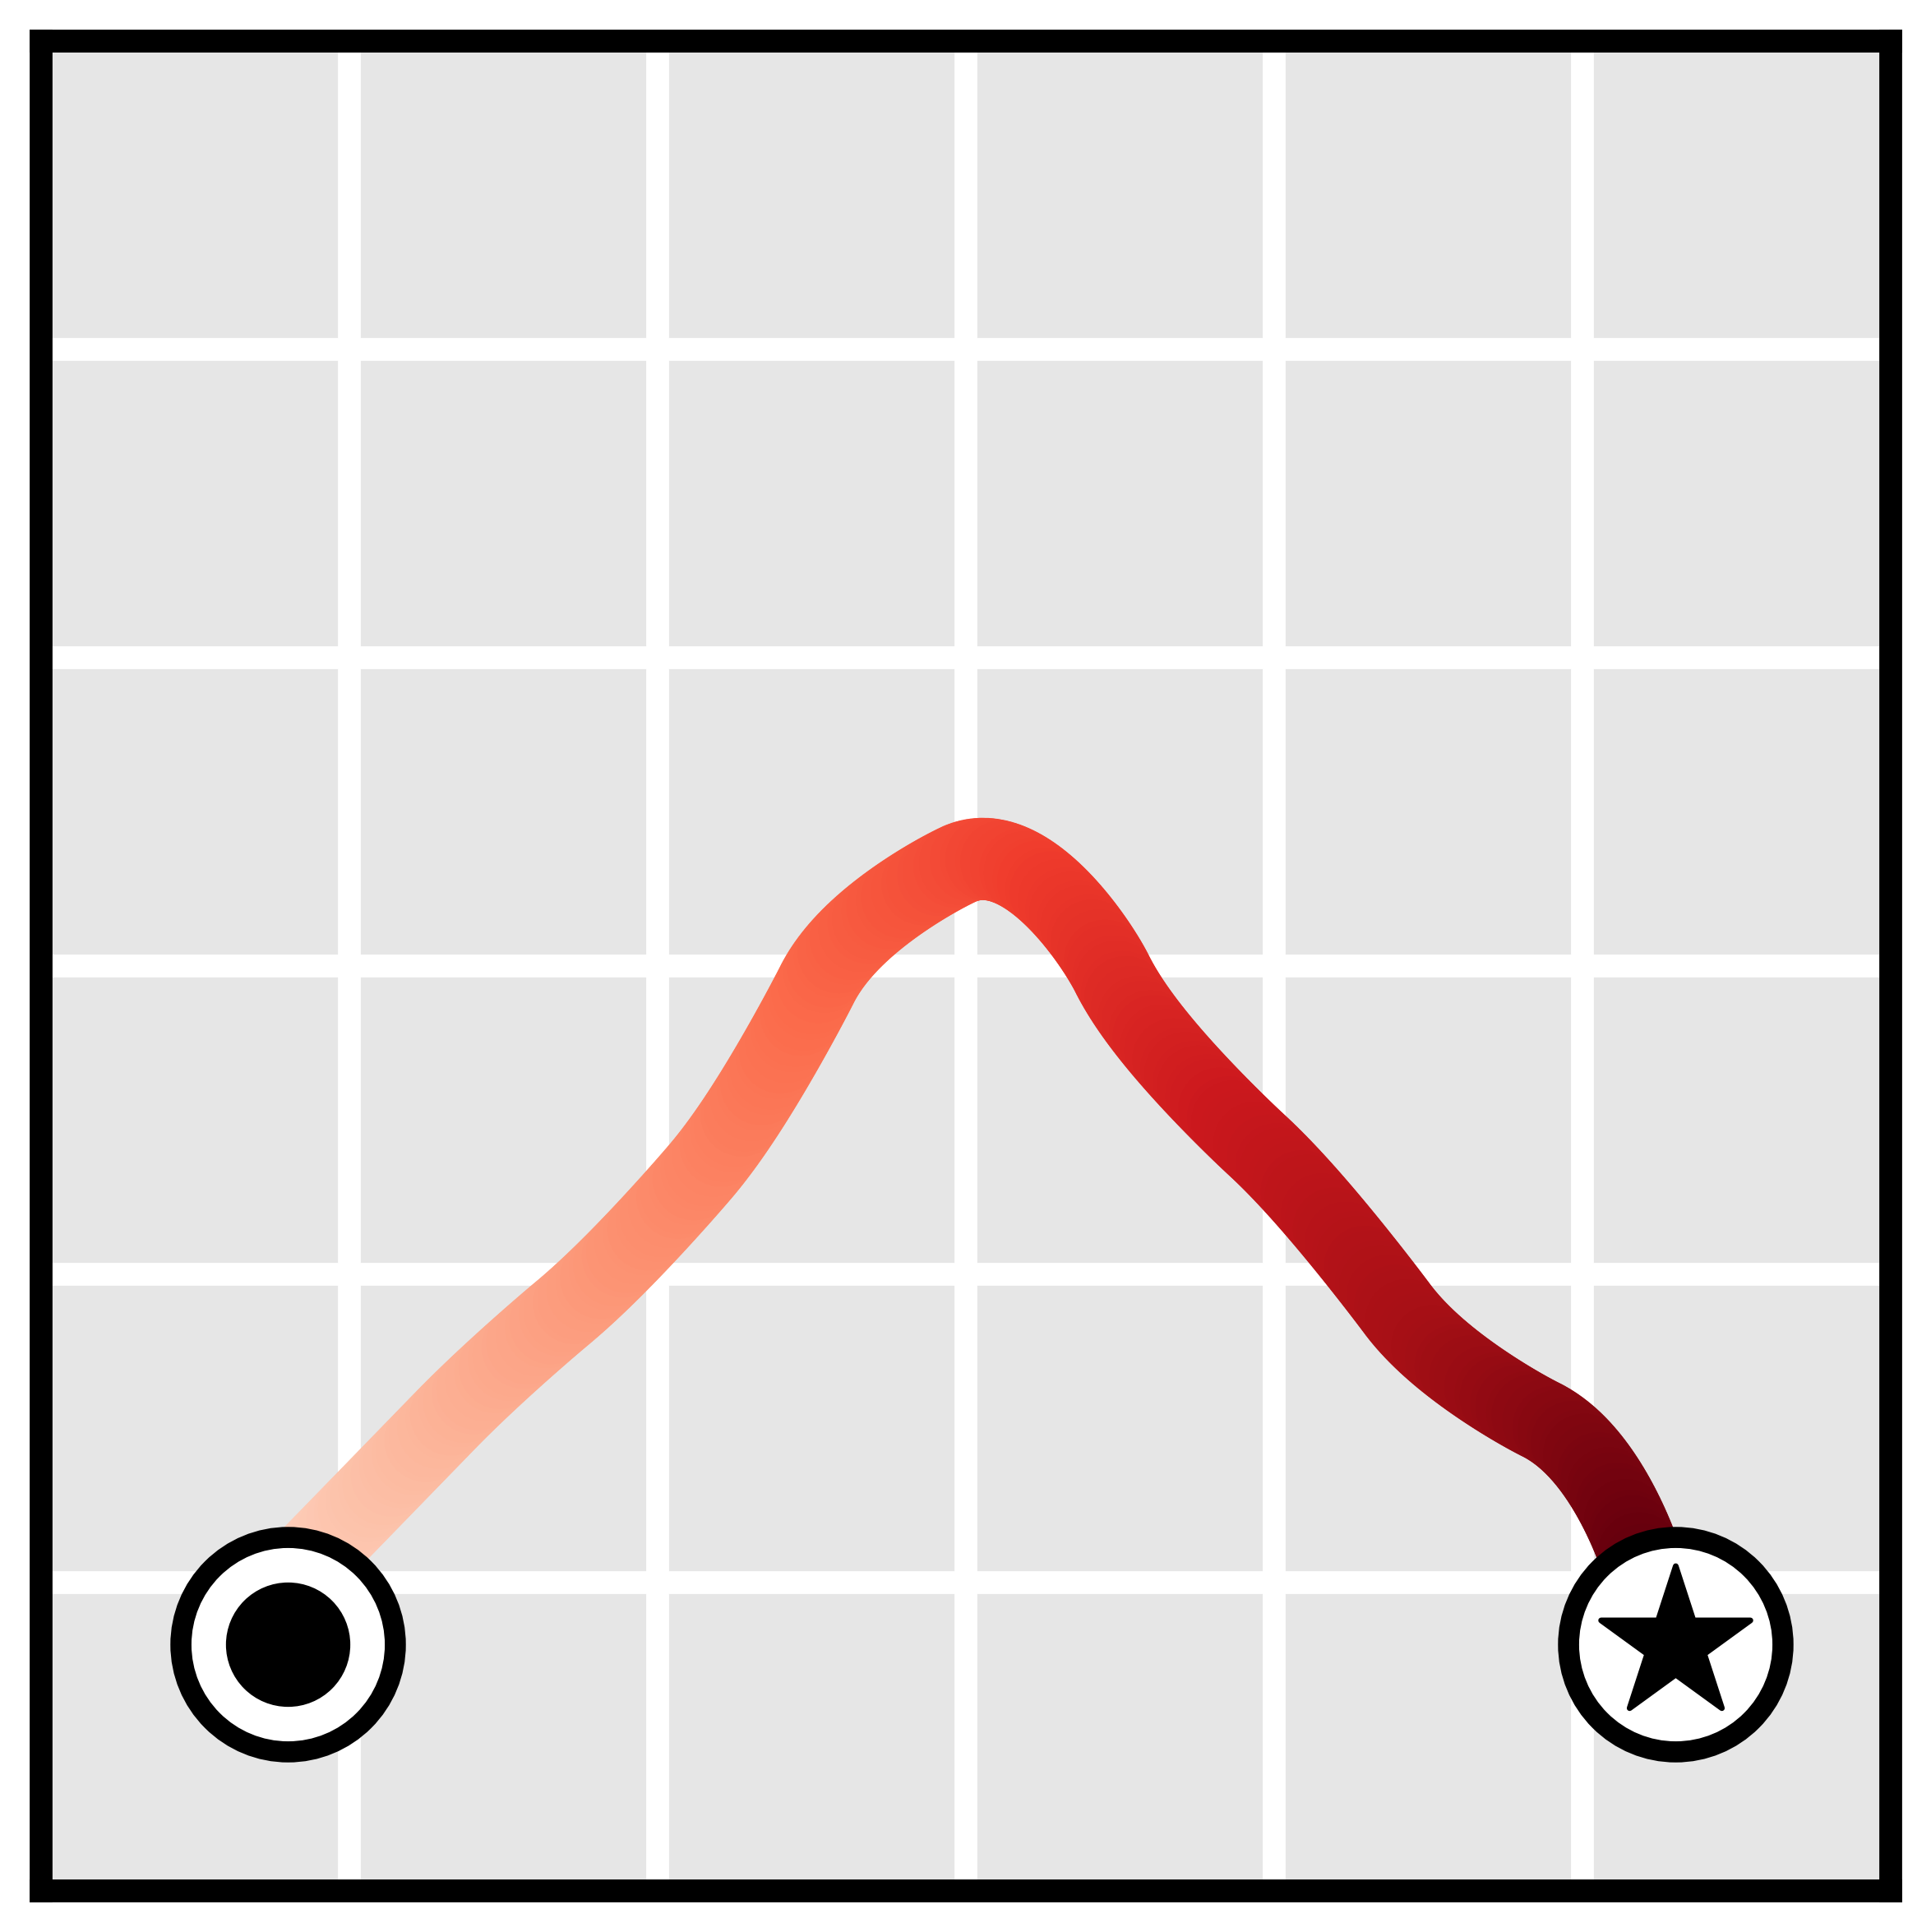
\includegraphics[width=2.5cm]{images/properties/stitching_plan.png} \\
    \vspace{-.5cm}
    \begin{center}
            \hspace{0.1cm} data \hspace{1.8cm} plan \\
    \end{center}
\end{minipage} \\
\vspace{.4cm}
%%%%
\begin{minipage}[t]{0.55\textwidth}
    \raisebox{2cm}{\textbf{c}}~~~
    \raisebox{0.3cm}{\undersetimage{images/properties/rand_0.png}{$\btau{N}$}{-0.25}}
        \raisebox{1.2cm}{$\rightarrow$}
        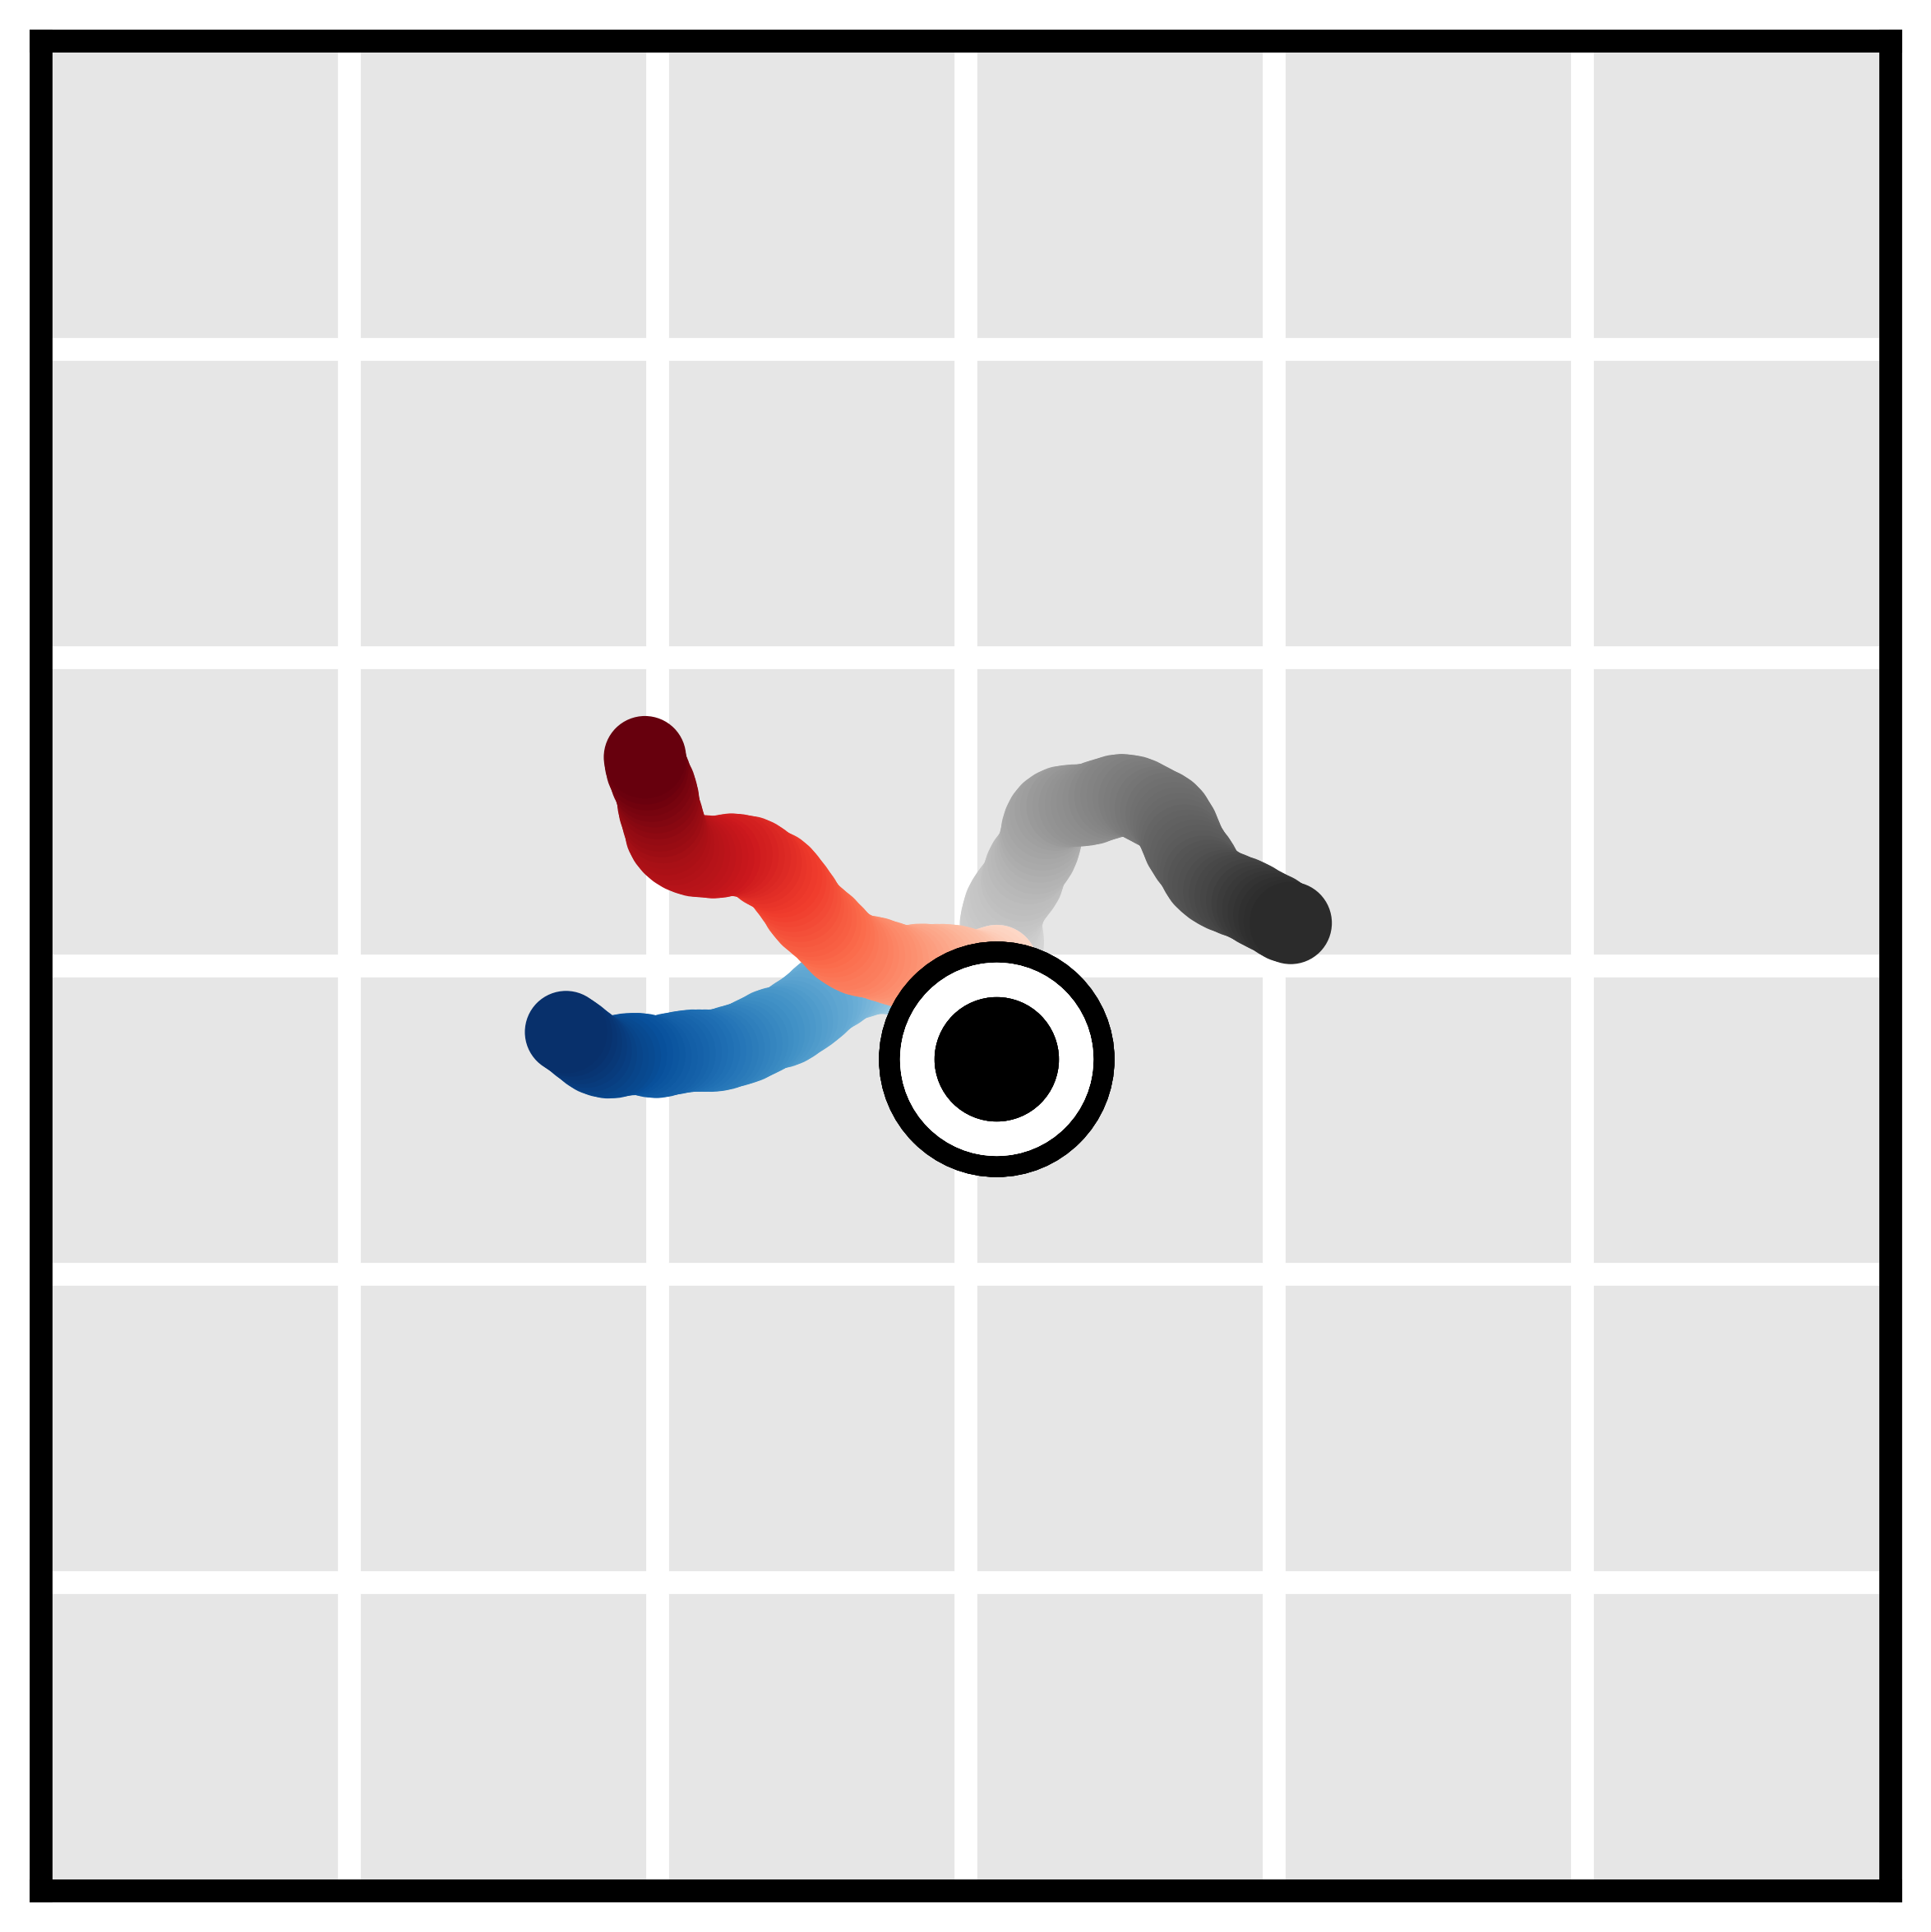
\includegraphics[width=2.5cm]{images/properties/variable_0.png}
        ~~
    \raisebox{-0.1cm}{\undersetimage{images/properties/rand_1.png}{$\btau{N}$}{-0.15}}
        \raisebox{1.2cm}{$\rightarrow$}
        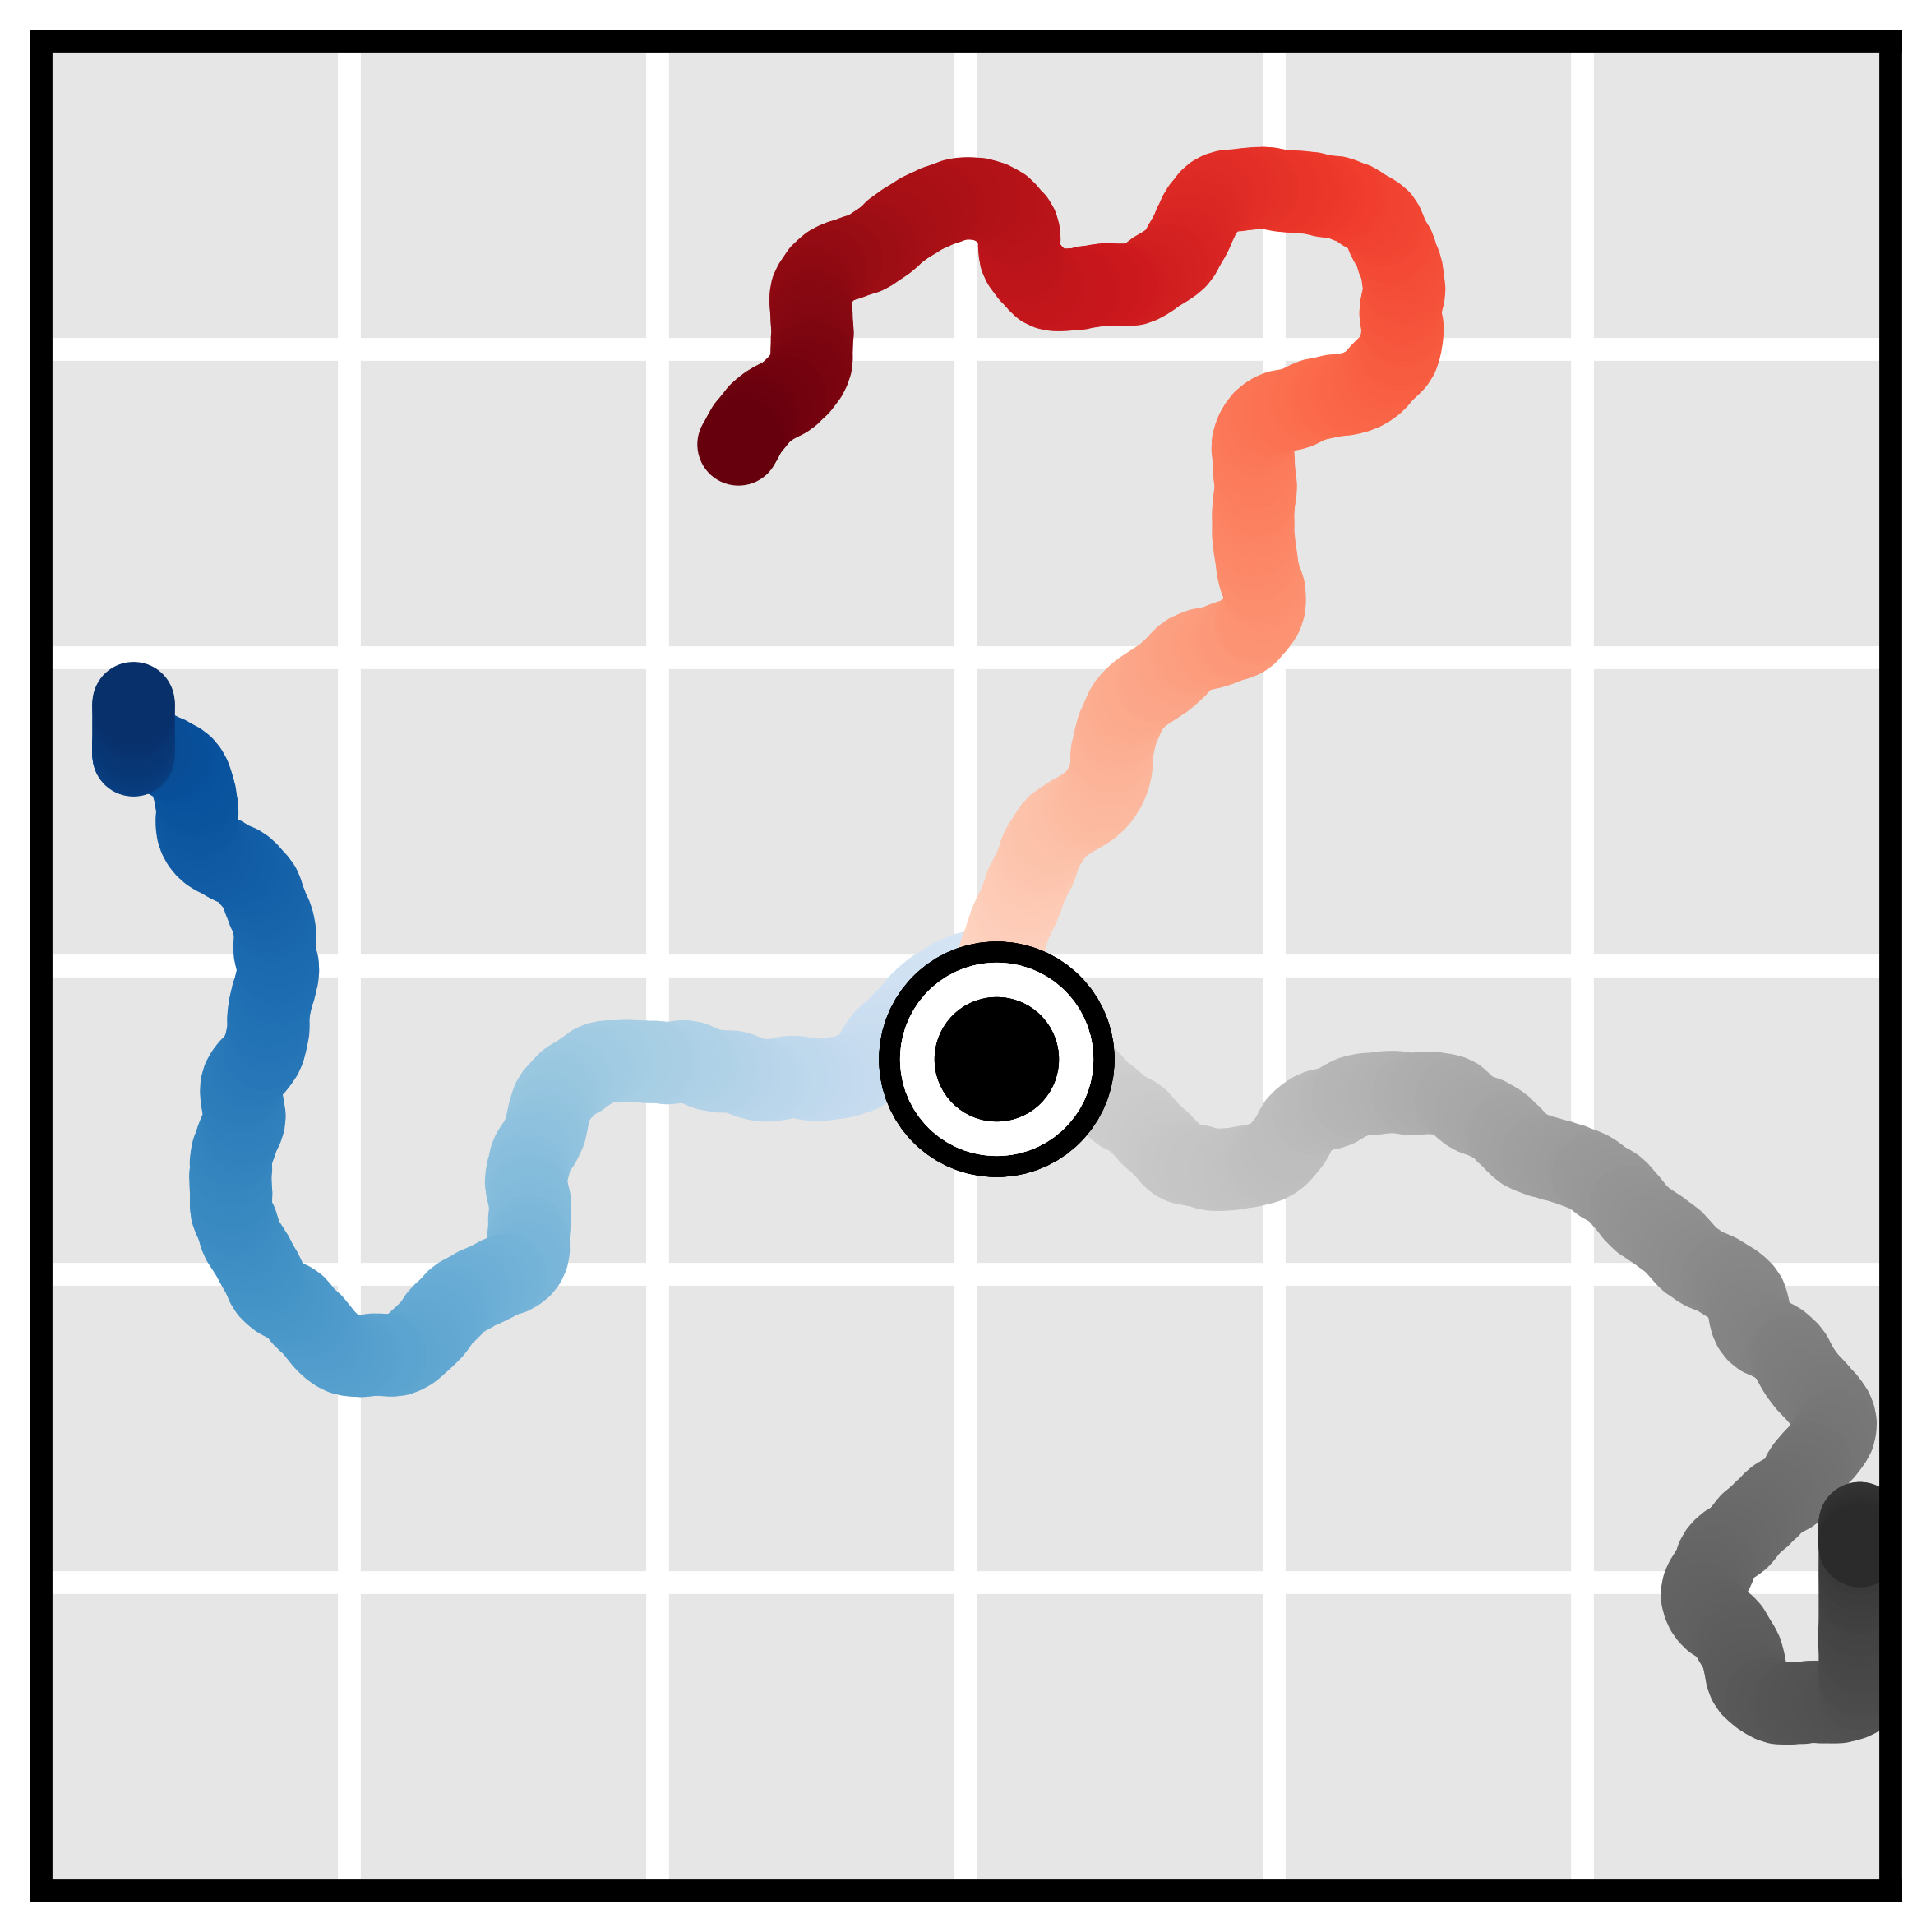
\includegraphics[width=2.5cm]{images/properties/variable_1_3.png} \\
    % ~~~~\raisebox{2cm}{$\btau{N}$} \\
\end{minipage}%
%%%%
\begin{minipage}[t]{0.35\textwidth}
    \raisebox{2cm}{\textbf{d}}~~~
    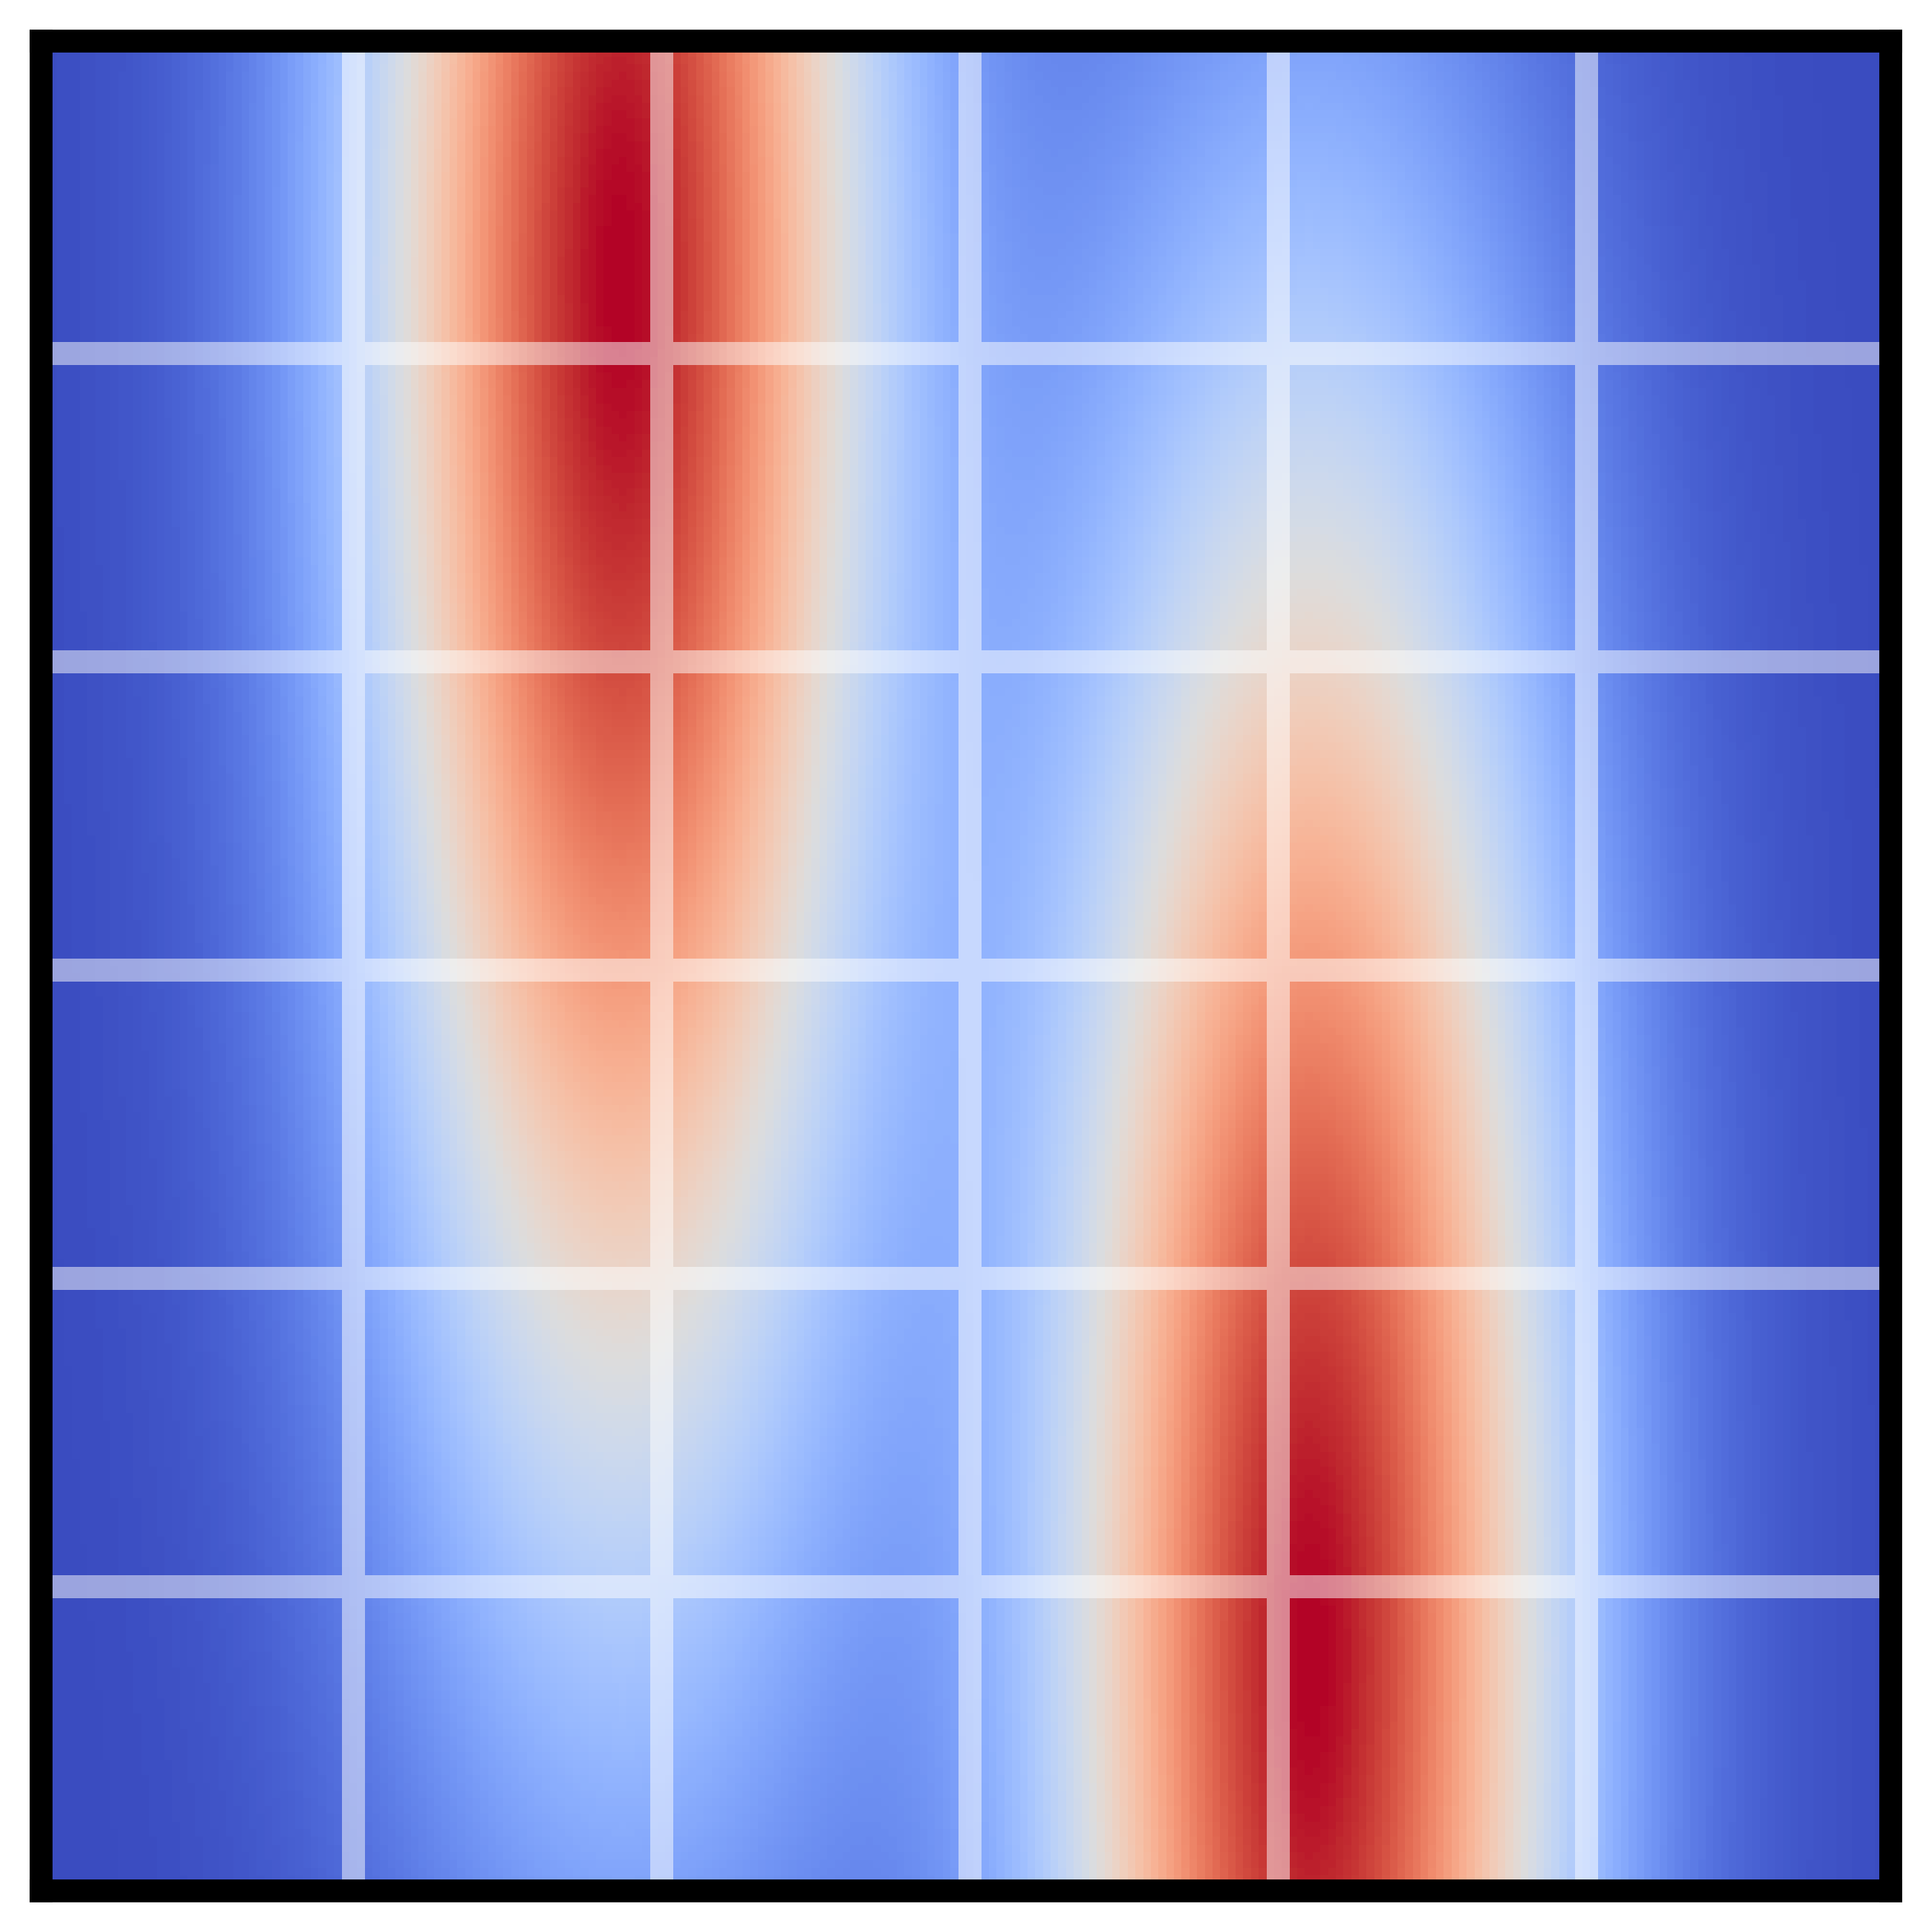
\includegraphics[width=2.5cm]{images/properties/reward.png}~
    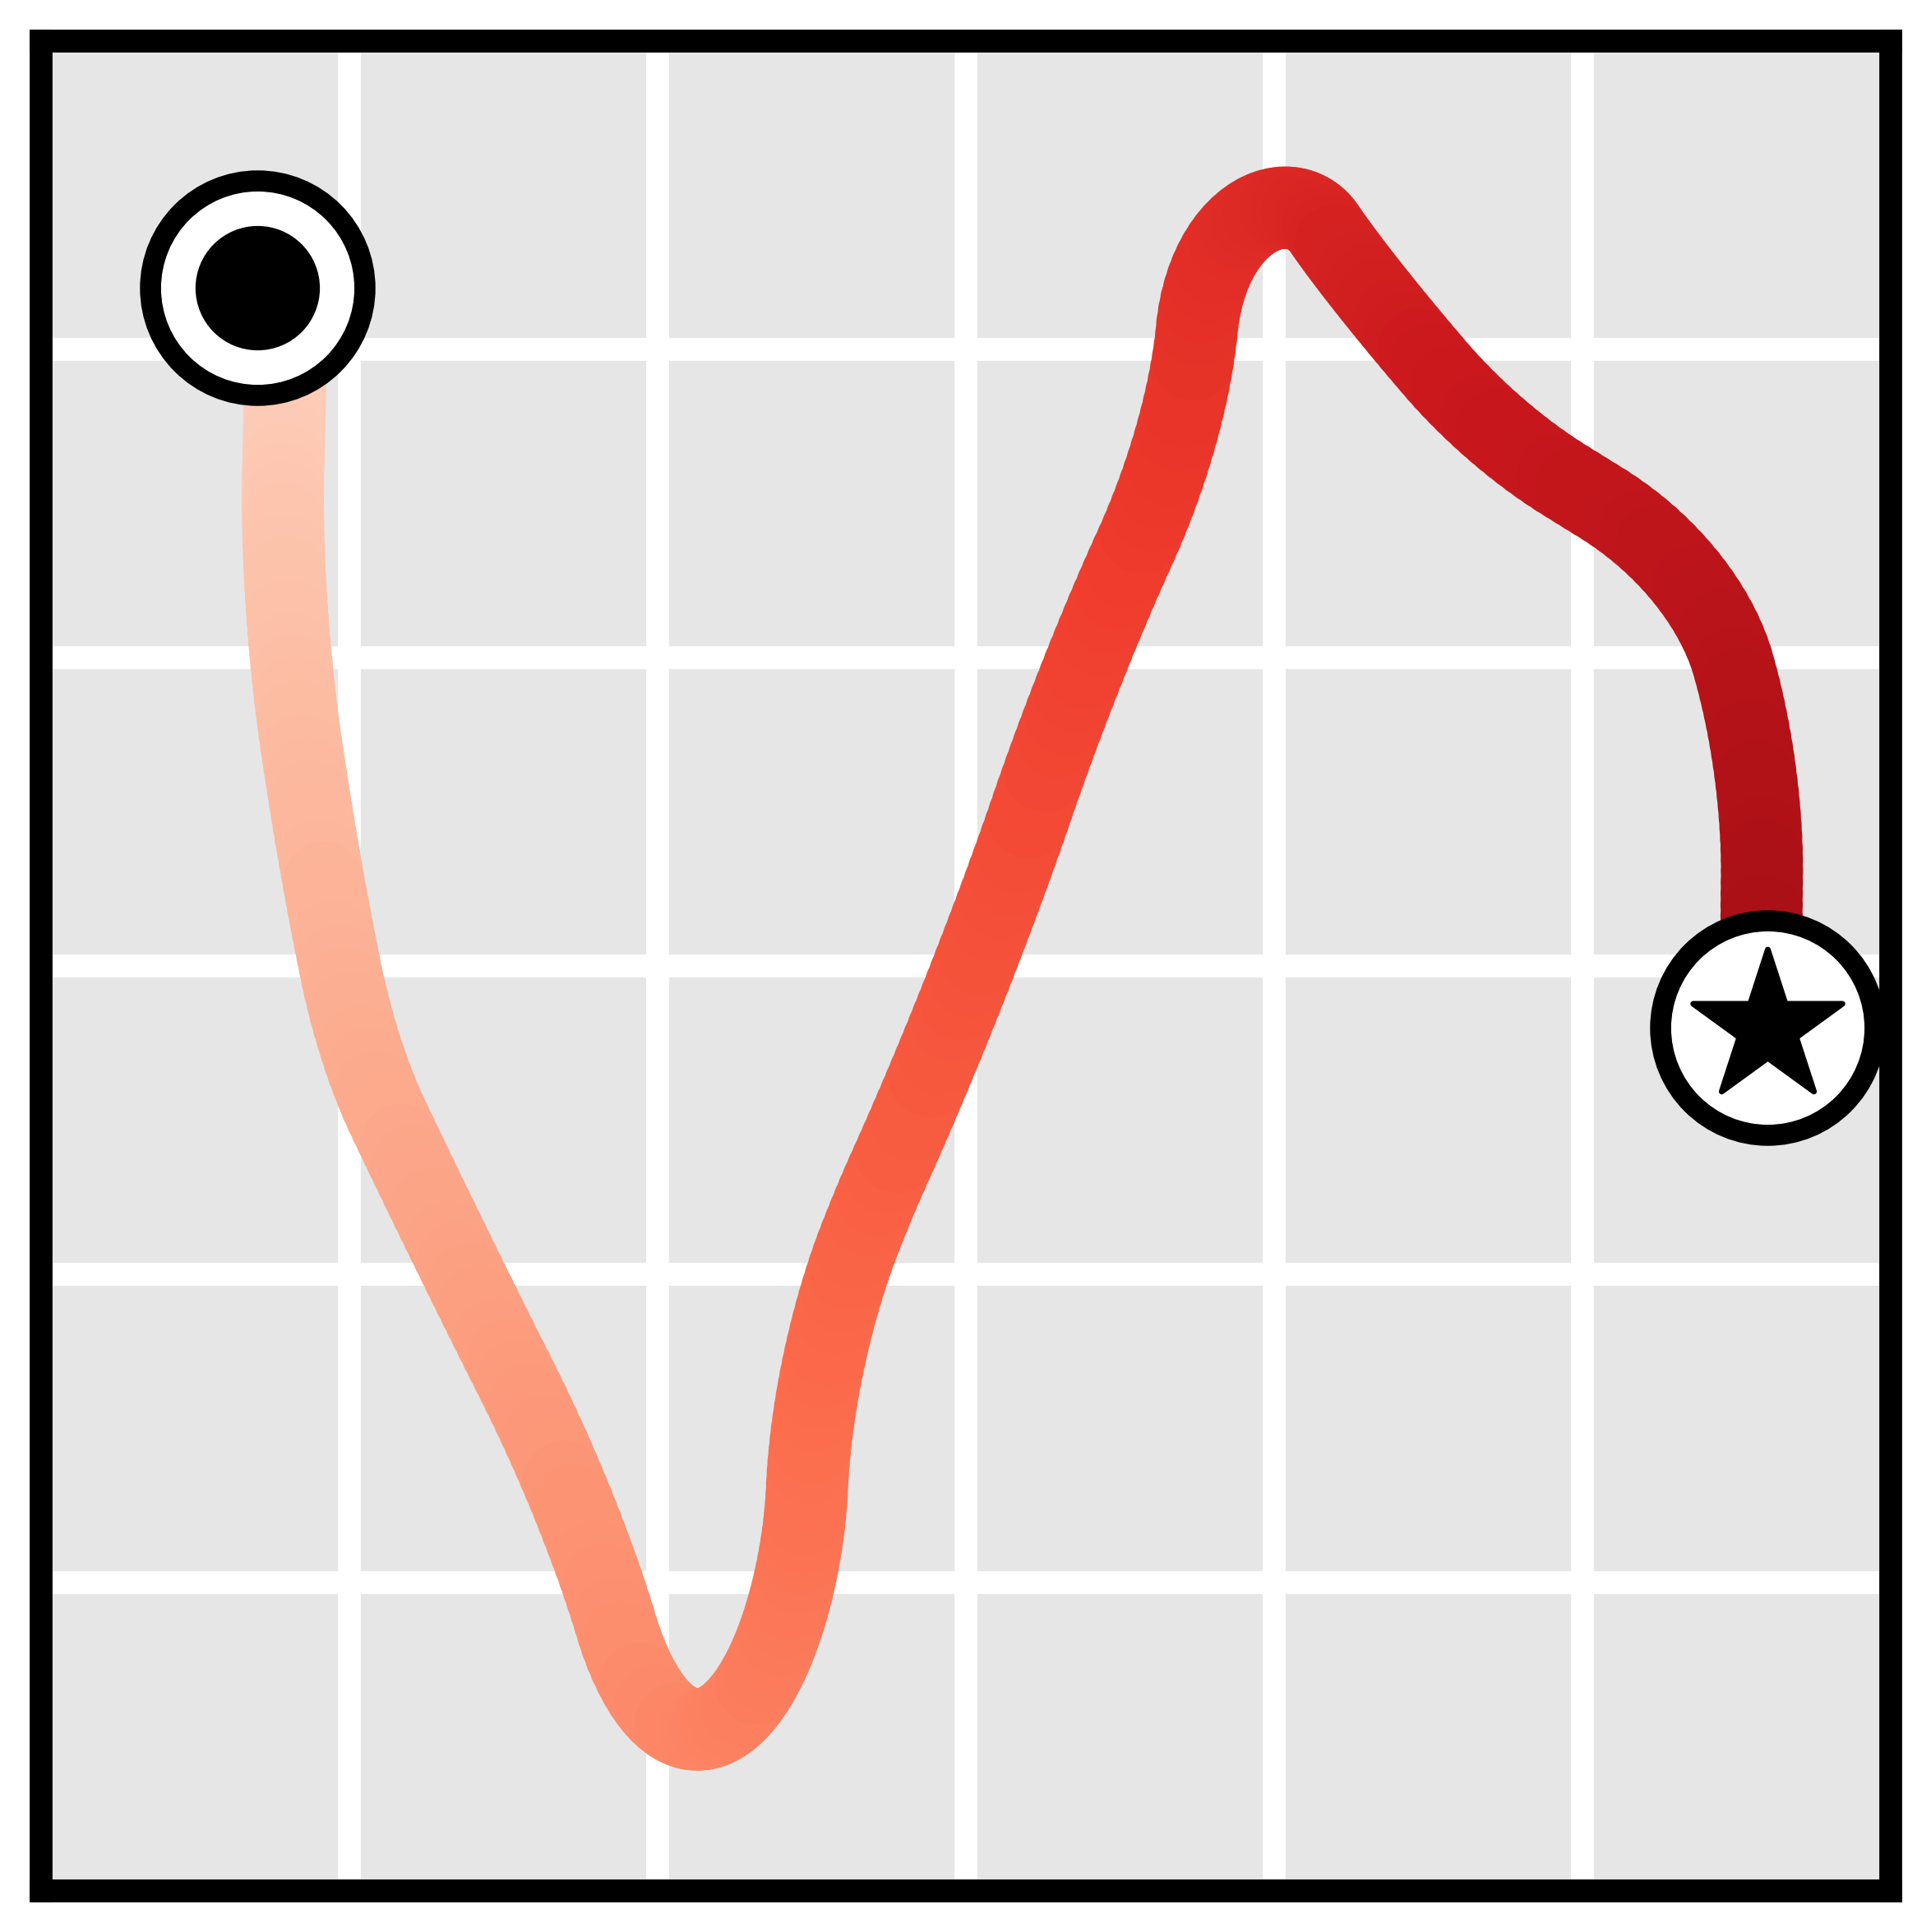
\includegraphics[width=2.5cm]{images/properties/reward_plan.png} \\
    \vspace{-.5cm}
    \begin{flushleft}
            \hspace{0.43cm} reward
            \hspace{0.0cm}
            \raisebox{.05cm}{$-$}
            \raisebox{.0cm}{
\includegraphics[height=1cm,angle=90]{images/properties/reward_colorbar.png}}
            \raisebox{.05cm}{$+$}
            \hspace{0.6cm} plan \\
    \end{flushleft}
\end{minipage}
\caption{
    % \small
    \textbf{(Properties of diffusion planners)}
    \textbf{(a) Learned long-horizon planning:}
    \method{}'s learned planning procedure does not suffer from the myopic failure modes common to shooting algorithms and is able to plan over long horizons with sparse reward.
    \textbf{(b) Temporal compositionality:} Even though the model is not Markovian, it generates trajectories via iterated refinements to local consistency.
    As a result, it exhibits the types of generalization usually associated with Markovian models, with the ability to stitch together snippets of trajectories from the training data to generate novel plan.
    \textbf{(c) Variable-length plans:}
    Despite being a trajectory-level model, \method's planning horizon is not determined by its architecture.
    The horizon can be updated after training by changing the dimensionality of the input noise.
    \textbf{(d) Task compositionality:} \method{} can be composed with new reward functions to plan for tasks unseen during training.
    In all subfigures,
    \protect{\raisebox{-.05cm}{
\includegraphics[height=.35cm]{images/maze2d/mark_start_crop.png}}}
    denotes a starting state and
    \protect{\raisebox{-.05cm}{
\includegraphics[height=.35cm]{images/maze2d/mark_goal_crop.png}}}
    denotes a goal state.
}
% \vspace{-.1cm}
\label{fig:properties}
% \vspace{-10pt}
\end{figure*}